%
% File acl2015.tex
%
% Contact: car@ir.hit.edu.cn, gdzhou@suda.edu.cn
%%
%% Based on the style files for ACL-2014, which were, in turn,
%% Based on the style files for ACL-2013, which were, in turn,
%% Based on the style files for ACL-2012, which were, in turn,
%% based on the style files for ACL-2011, which were, in turn, 
%% based on the style files for ACL-2010, which were, in turn, 
%% based on the style files for ACL-IJCNLP-2009, which were, in turn,
%% based on the style files for EACL-2009 and IJCNLP-2008...

%% Based on the style files for EACL 2006 by 
%%e.agirre@ehu.es or Sergi.Balari@uab.es
%% and that of ACL 08 by Joakim Nivre and Noah Smith

\documentclass[11pt]{article}
\usepackage{acl2015}
\usepackage{times}
\usepackage{url}
\usepackage{latexsym}
\usepackage{amsmath}
\usepackage{graphicx}

%\setlength\titlebox{5cm}

% You can expand the titlebox if you need extra space
% to show all the authors. Please do not make the titlebox
% smaller than 5cm (the original size); we will check this
% in the camera-ready version and ask you to change it back.


\title{Saracasm Detection Project}

\author{Leqi Liu \\
  Université Paris-Saclay, \\
  {\tt leqi.liu@etu-upsaclay.fr} \\\And
    Jiren Ren \\
   Université Paris-Saclay, \\
  {\tt renjiren120@gmail.com} \\}

\date{12/02/2025}

\begin{document}
\maketitle
\begin{abstract}
Sarcasm detection is a challenging task in Natural Language Processing (NLP) due to its implicit nature, where the intended meaning often contrasts with the literal text. Accurately identifying sarcasm is crucial for sentiment analysis, opinion mining, and conversational AI. In this study, we employ FastText and Skip-Gram for word vectorization, leveraging its ability to capture subword information and enhance word representations. These embeddings are then applied to CNN and LSTM to evaluate their effectiveness in sarcasm classification. Besides, we use SVM as a baseline model for comparison to exemplify the ability of neural networks in distinguishing sarcastic texts. The study hypothesizes that LSTM will excel in detecting sarcasm due to its ability to capture long-range dependencies, while CNN may be effective in identifying localized sarcasm patterns. The results are expected to shed light on the strengths and limitations of each model, offering insights to improve sarcasm detection techniques.
\end{abstract}

\section{Introduction}
The ability to accurately detect sarcasm can enhance AI's interpretative skills in various applications, such as social media analysis, chatbot interactions, and humor recognition.

With the advancement of deep learning and large-scale language models, sarcasm detection has gained significant research attention. Recent approaches leverage transformer-based architectures, such as BERT and GPT, to better grasp the implicit nature of sarcasm. Additionally, AI-generated sarcastic expressions can be used to improve training datasets, helping models better understand and generate nuanced responses. This can lead to more sophisticated conversational AI, capable of engaging in humor-driven interactions and understanding complex emotional contexts.

By improving sarcasm detection, NLP models can become more adept at reasoning about implicit information, ultimately enhancing their adaptability to fields like literary analysis, customer sentiment analysis, and humor recognition. This project explores various techniques to build a robust sarcasm detection model and investigates how AI can be trained to recognize and even generate sarcastic expressions for improved language understanding.

\section{Methods}
In this study, we build upon the work of \emph{Fracking Sarcasm using Neural Networks} \cite{ghosh2016magnets}, who explored sarcasm detection using neural networks without explicit word vectorization techniques. Unlike their approach, we utilize FastText and Skip-Gram to vectorize the words and compare its effectiveness in sarcasm detection. FastText enables our models to capture subword information, making it particularly useful for handling informal and creative sarcastic expressions. We apply these embeddings to CNN and LSTM. Besides, we use SVM as a baseline model for comparison to exemplify the ability of neural networks in distinguishing sarcastic texts.

By leveraging word vectorization, our study seeks to determine whether explicitly learned embeddings enhance sarcasm detection compared to previous neural network approaches. Through empirical evaluation, we aim to provide insights into the advantages and limitations of different architectures and contribute to the development of more effective sarcasm detection models.

\section{Dataset}
For this sarcasm detection task, we used a dataset sourced from the reference \emph{Fracking Sarcasm using Neural Networks} \cite{ghosh2016magnets}. The dataset consists of labeled Twitter data, where each tweet is categorized as either sarcastic or non-sarcastic. This dataset is specifically curated for sarcasm detection in informal, social media-based text, making it highly suitable for our task, given the nature of sarcasm in such contexts.

The dataset contains a total of 54,931 samples, each of which is a tweet. The labels are binary, with 1 indicating sarcasm and 0 indicating non-sarcasm. This provides a clear and well-defined classification task, where the model learns to distinguish between sarcastic and non-sarcastic expressions based on the language patterns observed in the tweets.

\begin{table}[ht]
\centering
\begin{tabular}{|c|c|}
\hline
\multicolumn{2}{|c|}{\textbf{Train Set}} \\ \hline
Sarcastic & Non-sarcastic \\ \hline
24,453 & 26,736 \\ \hline
\multicolumn{2}{|c|}{\textbf{Test Set}} \\ \hline
Sarcastic & Non-sarcastic \\ \hline
1,419 & 2,323 \\ \hline
\end{tabular}
\caption{Dataset Split}
\end{table}

In detail, the dataset is constructed by collecting tweets that explicitly contain the \texttt{\#sarcasm} hashtag as a retrieval cue. Since relying solely on this heuristic might overlook sarcastic tweets without such explicit markers, the list of indicative hashtags is expanded using an \textbf{LSA-based approach}, incorporating tags like \texttt{\#sarcastic}, \texttt{\#yeahright}, and other related terms. Additionally, tweets from users with a strong inclination toward either sincerity or sarcasm (e.g., professional comedians) are included to enhance dataset quality.

Unlike previous works, we used \textbf{SVM} as our baseline classification model and used Skip-Gram and Fasttext for word embeddings. Initially, we conducted experiments on smaller subsets (\texttt{train\_sample} and \texttt{test\_sample}) to validate our approach before applying it to the full \texttt{train} and \texttt{test} sets.

\section{Data Preprocessing}
In \textbf{data preprocessing}, we made several works:
\begin{enumerate}
    \item All \texttt{@mentions} were replaced with \texttt{@user} to anonymize user references.
    \item Any hashtag matching the pattern \texttt{\#sarca*} (e.g., \texttt{\#sarcasm}, \texttt{\#sarcastic}) was removed to prevent direct labeling bias.
    \item \textbf{Stopwords} and \textbf{URLs} were filtered out to improve model focus on key linguistic features.
    \item All \textbf{emojis} were replaced with its meaning in English.
    \item All verbs and nouns are \textbf{lemmatized}.
\end{enumerate}

These preprocessing steps ensured a cleaner, more generalized input for sarcasm detection while maintaining the essential context of the tweets.

\section{SVM}
Support Vector Machines (SVM) are a well-established machine learning approach that is effective in high-dimensional spaces, making it suitable for text classification tasks. In our experiment, we used SVM with a linear kernel, leveraging the Term Frequency-Inverse Document Frequency (TF-IDF) representation of text. The TF-IDF features were extracted to capture the importance of words relative to the entire corpus, and the linear kernel was chosen for its simplicity and efficiency.

Mathematically, the SVM objective is to find a hyperplane $\textbf{w}^T\textbf{x}+b=0$ that maximizes the margin between the two classes. The optimization problem is formulated as:

\begin{align}
    &\min_{\textbf{w},b,\xi_i}\frac{1}{2}||\textbf{w}||^2+C\sum_{i=1}^N\xi_i \\
    &\text{s.t. }y_i(\textbf{w}^T\textbf{x}_i+b)\geq 1-\xi_i,\ \xi_i\geq 0 \notag
\end{align}
where $\xi_i$ are slack variables that allow some margin violations, and $C$ is the regularization parameter. The goal is to separate sarcastic and non-sarcastic classes in the feature space, ensuring the best possible margin between them.

\section{Neural Network}
\subsection{CNN}
Convolutional Neural Networks (CNNs) have demonstrated great success in capturing local dependencies in data, particularly in tasks where spatial hierarchies or local feature patterns are significant. In the context of sarcasm detection, CNNs are effective at identifying the short-range relationships between words and phrases, which are often key to understanding the sarcastic tone. The CNN model was designed to learn spatial patterns in the text that reflect sarcastic sentiments, such as reversal of sentiment or ironic expressions, through local contextual cues.

\subsection{LSTM}
Long Short-Term Memory (LSTM) networks are a type of Recurrent Neural Network (RNN) that are particularly effective at modeling sequential data with long-range dependencies.\cite{lstm} Given an input sequence $\textbf{X}=\{\textbf{x}_1,\textbf{x}_2,...,\textbf{x}_T\}$, where $\textbf{x}_t$ is the word embedding at time step $t$, the LSTM uses gating mechanisms to control the flow of information.

\begin{itemize}
    \item Forget Gate: Decides what information to discard from the cell state:
    \begin{align}
        f_t=\sigma(W_f\cdot[\textbf{h}_{t-1},\textbf{x}_t]+b_f)
    \end{align}
    \item Input Gate: Determines which values to update in the cell state:
    \begin{align}
        i_t=\sigma(W_i\cdot[\textbf{h}_{t-1},\textbf{x}_t]+b_i)
    \end{align}
    \begin{align}
        \tilde{C}_t=\tanh(W_C\cdot[\textbf{h}_{t-1},\textbf{x}_t]+b_C)
    \end{align}
    \item Cell State Update: Updates the cell state based on the forget and input gates:
    \begin{align}
        C_t=f_t*C_{t-1}+i_t*\tilde{C}_t
    \end{align}
    \item Output Gate: Decides what the next hidden state should be:
    \begin{align}
        o_t=\sigma(W_o\cdot[\textbf{h}_{t-1},\textbf{x}_t]+b_o)
    \end{align}
    \begin{align}
        \textbf{h}_t=o_t*\tanh(C_t)
    \end{align}
\end{itemize}

In sarcasm detection, the understanding of sarcastic intent often requires considering the broader context, which can span multiple sentences or phrases. LSTMs, with their gating mechanisms, are able to retain long-term information and mitigate issues like vanishing gradients in traditional RNNs.

We used pre-trained word embeddings to represent the text input, which were then processed by the LSTM layers to capture the sequential relationships between words in the context of sarcasm. A fully connected layer at the output stage was used to classify the final representation into sarcastic or non-sarcastic categories. The LSTM model is capable of learning complex patterns that involve shifts in meaning and sentiment, which are characteristic of sarcastic statements.

\section{Experimental Setup}
We employed an SVM with a linear kernel as our baseline model. The linear kernel was chosen for its simplicity and computational efficiency. No hyperparameter optimization was performed for the SVM; it was trained using default settings. The SVM model serves as a straightforward comparison to more complex models, helping to highlight the improvements gained from using deep learning architectures. 

For the CNN, we designed a multi-layer architecture with one-dimensional convolutional layers. The input to the network consisted of word embeddings (either SkipGram or FastText) fed into an embedding layer. The CNN was trained using the Adam optimizer with a learning rate of 0.001, and we used dropout regularization to mitigate overfitting.

The LSTM model aimed to capture long-range dependencies within the text. Similar to the CNN, the input to the LSTM was word embeddings, which were passed through an embedding layer before entering the LSTM network. The LSTM consisted of a single layer with 128 units. We used the Adam optimizer with a learning rate of 0.001 and applied dropout (0.5) to prevent overfitting.

The code of SVM and neural network was implemented using Sklearn and Pytorch library, respectively. And the code of word vectorization was implemented using Gensim.

\section{Experimental Analysis}
The models were evaluated using standard classification metrics, including accuracy, precision, recall, and F1-score. We focused on maximizing the F1-score to balance the model’s performance in identifying both sarcastic and non-sarcastic tweets. 

%这里可放SVM的两张图。
As shown in Figure \ref{fig:svmcr} and \ref{fig:svmcm}, SVM model demonstrates reasonable performance, particularly in detecting sarcastic instances (recall = 0.73). However, false positives (FP = 4) and false negatives (FN = 3) indicate that the classifier struggles to differentiate between sarcasm and non-sarcasm effectively.
\begin{figure}[htbp]
    \centering
    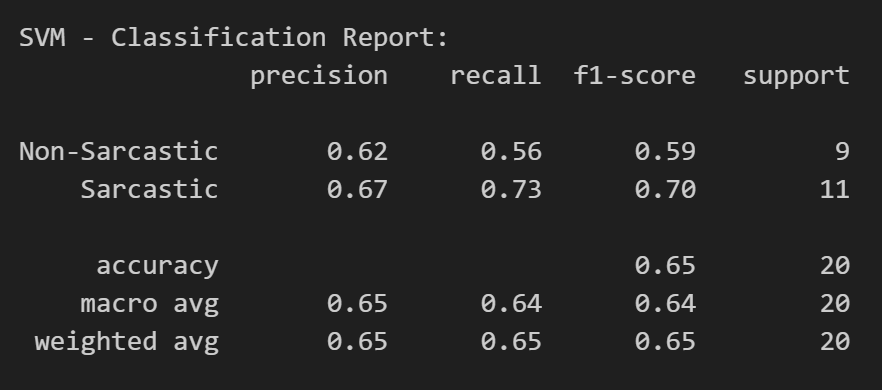
\includegraphics[width=.8\linewidth]{pic/SVM-Report.png}
    \caption{SVM Classification Report}
    \label{fig:svmcr}
\end{figure}
\begin{figure}[htbp]
    \centering
    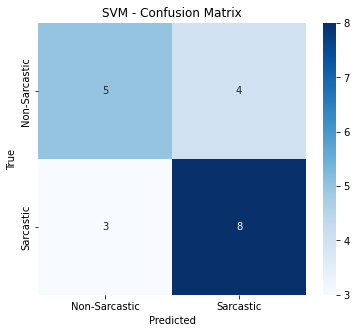
\includegraphics[width=.8\linewidth]{pic/SVM-Confusion-Matrix.png}
    \caption{Confusion Matrix of SVM}
    \label{fig:svmcm}
\end{figure}

%这里放CNNSKIPgram
As shown in Figure \ref{fig:sgcnncr} and \ref{fig:sgcnncm}, CNN model using Skip-Gram word vectorization has a better performance, especially in classifying non-sarcastic tweets. But it tends to classify sarcasm tweets to non-sarcasm tweets.
\begin{figure}[htbp]
    \centering
    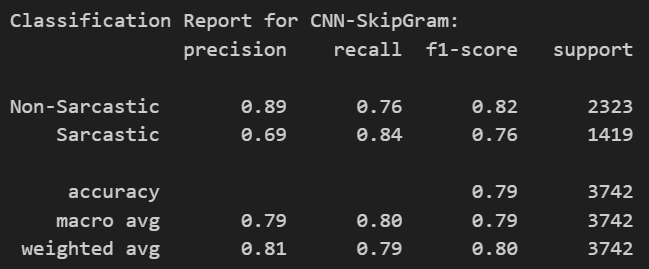
\includegraphics[width=.8\linewidth]{pic/CNN-Skipgram-Report.png}
    \caption{Skip-gram \& CNN Classification Report}
    \label{fig:sgcnncr}
\end{figure}
\begin{figure}[htbp]
    \centering
    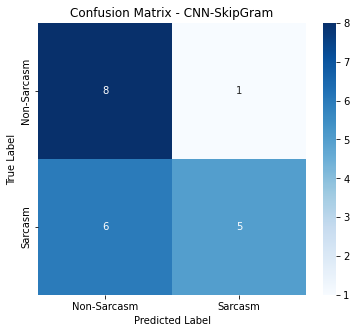
\includegraphics[width=.8\linewidth]{pic/CNN-skipgram-Matrix.png}
    \caption{Confusion Matrix of Skip-gram \& CNN}
    \label{fig:sgcnncm}
\end{figure}

%CNN fasttext
As shown in Figure \ref{fig:ftcnncr} and \ref{fig:ftcnncm}, CNN model using Fasttext word vectorization is worse than CNN using Skip-Gram. Plenty of sarcastic tweets are classified to be non-sarcastic. Compared to CNNs using Skip-Gram, Fasttext does not provide better word vectors to reveal the connections behind words that may be indicative of sarcasm.
\begin{figure}[htbp]
    \centering
    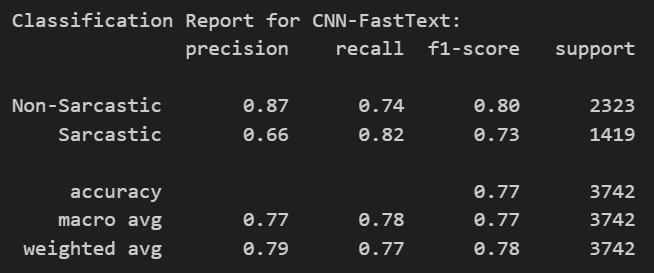
\includegraphics[width=.8\linewidth]{pic/CNN-fasttext-Report.png}
    \caption{Fasttext \& CNN Classification Report}
    \label{fig:ftcnncr}
\end{figure}
\begin{figure}[htbp]
    \centering
    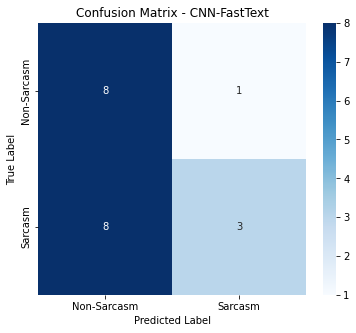
\includegraphics[width=.8\linewidth]{pic/CNN-fasttext-Matrix.png}
    \caption{Confusion Matrix of Fasttext \& CNN}
    \label{fig:ftcnncm}
\end{figure}

%LSTM SJIP-GRAM
As shown in Figure \ref{fig:sglstmcr} and \ref{fig:sglstmcm}, among all the models, the LSTM model using Skip-Gram word vectorization performed the best with the highest accuracy of 0.70.
\begin{figure}[htbp]
    \centering
    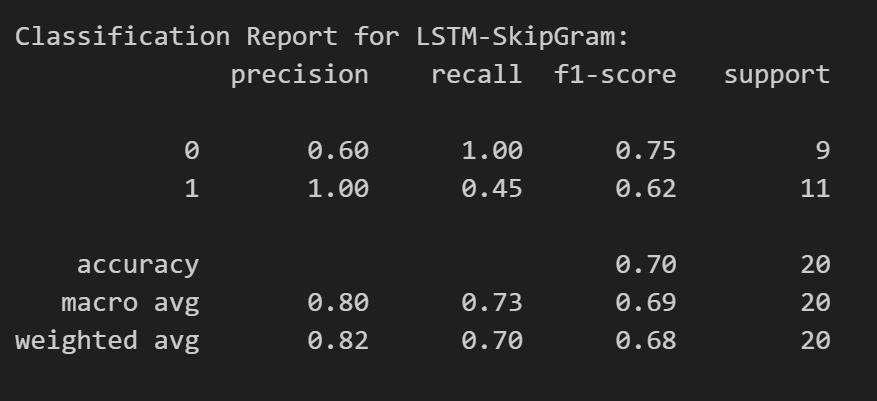
\includegraphics[width=.8\linewidth]{pic/LSTM-Skipgram-Report.png}
    \caption{Skip-gram \& LSTM Classification Report}
    \label{fig:sglstmcr}
\end{figure}
\begin{figure}[htbp]
    \centering
    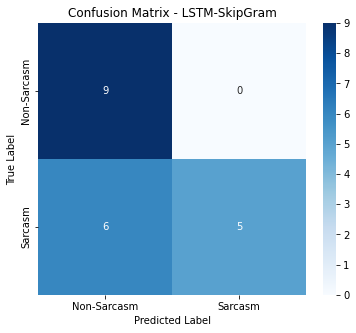
\includegraphics[width=.8\linewidth]{pic/LSTM-skipgram-Matrix.png}
    \caption{Confusion Matrix of Skip-gram \& LSTM}
    \label{fig:sglstmcm}
\end{figure}

%LSTM FASTTEXT
As shown in Figure \ref{fig:ftlstmcr} and \ref{fig:ftlstmcm}, LSTM model using Fasttext word vectorization is weaker in classifying non-sarcastic tweets but a bit better in sarcastic tweets compared with LSTM skip-gram.
\begin{figure}[htbp]
    \centering
    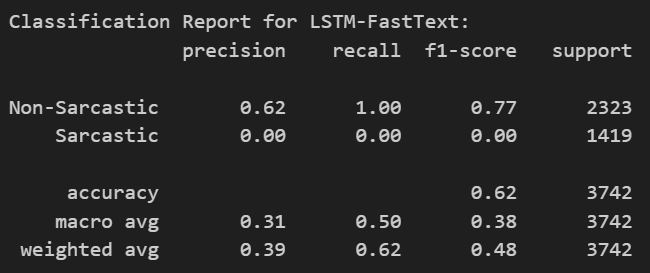
\includegraphics[width=.8\linewidth]{pic/LSTM-fasttext-Report.png}
    \caption{Fasttext \& LSTM Classification Report}
    \label{fig:ftlstmcr}
\end{figure}
\begin{figure}[htbp]
    \centering
    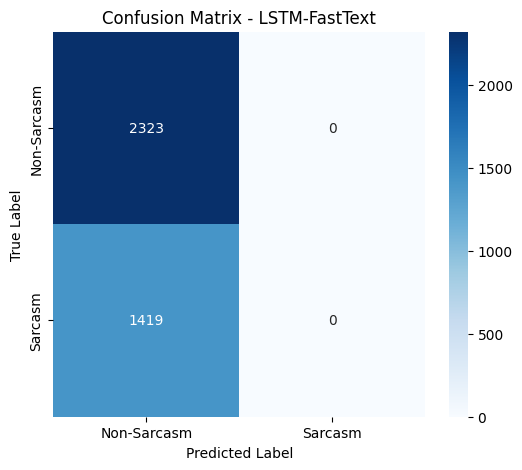
\includegraphics[width=.8\linewidth]{pic/LSTM-fasttext-Matrix.png}
    \caption{Confusion Matrix of Fasttext \& LSTM}
    \label{fig:ftlstmcm}
\end{figure}

%comparison图
Figure \ref{fig:comp} is the comparison plot of the 4 scores for the different models. The accuracy scores are not provided in the references, so the bars for accuracy are missing from the plot. From the references and our research results, we found that deep learning models work better than simple machine learning models such as SVMs, especially LSTM using Skip-Gram works best because this task focuses more on contextual information rather than partial and isolated information.
\begin{figure}[htbp]
    \centering
    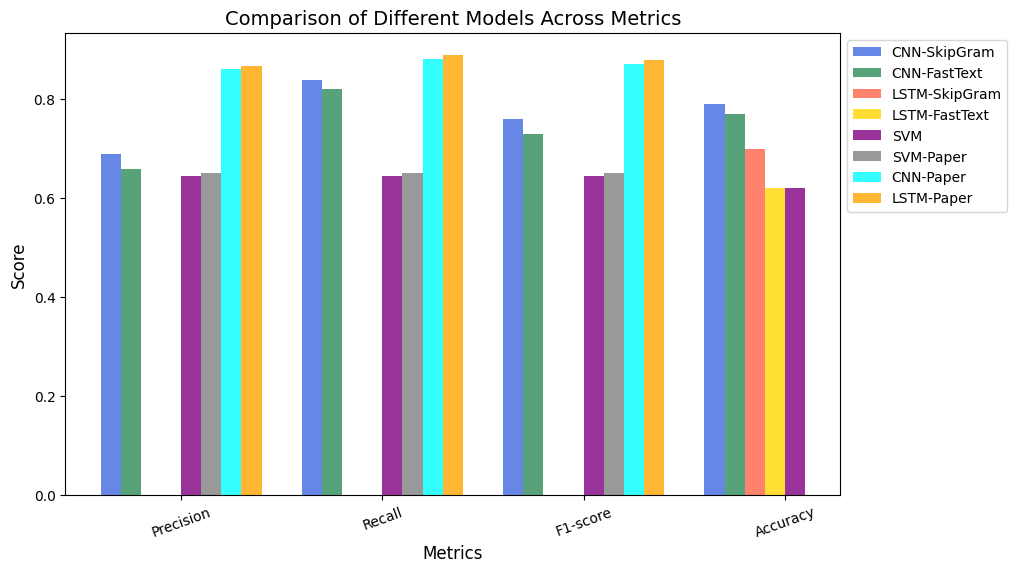
\includegraphics[width=\linewidth]{pic/Comparison.png}
    \caption{Comparison of the 4 scores for the different models}
    \label{fig:comp}
\end{figure}

However, we were unable to obtain results as good as those in the references due to the following reasons:
\begin{itemize}
    \item Because of poor CPU performance and the non-use of GPUs, the training and test sizes of the datasets we used were not as large as in references.
    \item There are some training tricks used in the code provided by the references.
    \item Some information of our tweets is disgarded during data preprocessing, such as the references kept all usernames while we not.
\end{itemize}

\section{Conclusion and Future work}
In this project, we tackled sarcasm detection using SVM, CNN, and LSTM models, along with word embeddings like SkipGram and FastText. Our experiments showed that LSTM outperformed the other models in capturing the contextual nuances of sarcasm, while Skip-Gram provided better handling of rare words. Although the models performed well, there is still room for improvement in dealing with more complex sarcastic contexts.

Future research could focus on exploring advanced models like Transformer and BERT, or employing ensemble techniques to further boost performance. Extending sarcasm detection to other languages, incorporating more contextual features such as sentiment or pragmatic cues, and using more diverse datasets would also help improve the model. Additionally, integrating multimodal data like images or audio could provide a more comprehensive understanding of sarcasm.

\section{Contributions}

\begin{table}[ht]
\centering
\begin{tabular}{|l|l|}
\hline
\textbf{Task}              & \textbf{Responsible Member} \\ \hline
Data Preprocessing         & Leqi Liu                    \\ \hline
Feature Extraction         & Leqi Liu \& Jiren Ren       \\ \hline
Model Construction         & Leqi Liu \& Jiren Ren       \\ \hline
Model Training \& Testing  & Leqi Liu \& Jiren Ren       \\ \hline
Data Visualization         & Jiren Ren                   \\ \hline
Final Report \& Slide      & Leqi Liu \& Jiren Ren       \\ \hline
\end{tabular}
\caption{Project Contributions}
\end{table}


% include your own bib file like this:
%\bibliographystyle{acl}
%\bibliography{acl2015}

\begin{thebibliography}{}

\bibitem[\protect\citename{Ghosh et al.}2016]{ghosh2016magnets}
Ghosh, A., \& Veale, D. T.
\newblock 2016.
\newblock Fracking Sarcasm using Neural Network.
\newblock {\em Proceedings of the 7th Workshop on Computational Approaches to Subjectivity, Sentiment and Social Media Analysis,}
\newblock pages 161–169, San Diego, California. Association for Computational Linguistics.

\bibitem[\protect\citename{Hochreiter et al.}1997]{lstm}
Hochreiter, S., \& Schmidhuber, J.
\newblock 1997.
\newblock Long short-term memory
\newblock {\em Neural computation}
\newblock 9(8):1735-1780.

\bibitem[\protect\citename{Kreuz et al.}2007]{lips}
Kreuz, R., \& Caucci, G.
\newblock 2007.
\newblock Lexical Influences on the Perception of Sarcasm.
\newblock {\em In Proceedings of the Workshop on Computational Approaches to Figurative Language,}
\newblock pages 1–4, Rochester, New York. Association for Computational Linguistics.

\bibitem[\protect\citename{Burfoot et al.}2009]{asd}
Burfoot, C., \& Baldwin, T.
\newblock 2009.
\newblock Automatic Satire Detection: Are You Having a Laugh?.
\newblock {\em In Proceedings of the ACL-IJCNLP 2009 Conference Short Papers,}
\newblock pages 161–164, Suntec, Singapore. Association for Computational Linguistics.

\bibitem[\protect\citename{Tungthamthiti et al.}2014]{rst}
Tungthamthiti, P., Shirai, K., \& Mohd, M.
\newblock 2014.
\newblock Recognition of Sarcasms in Tweets Based on Concept Level Sentiment Analysis and Supervised Learning Approaches.
\newblock {\em Pacific Asia Conference on Language, Information and Computation,}

\end{thebibliography}

\end{document}